\chapter{Hardware e Software Utilizados}

\section{Codificação e Testes}
\subsection{Ambiente de Desenvolvimento}
O ambiente para desenvolvimento da solução foi criado em um único computador, de caráter pessoal, do tipo notebook, com as seguintes especificações técnicas \cite{notebook-info}:
	\begin{itemize}
		\item Processador Intel Core i5 3230M - 2.60 GHz (T-Max: 3.20 GHz) - 64 Bits - Smart Cache 3 MB L3
	\end{itemize}
	\begin{itemize}
		\item Chipset Intel ® HM75 Express
	\end{itemize}
	\begin{itemize}
		\item Memória RAM 8 GBs DDR3 SDRAM - 1600 MHz
	\end{itemize}
	\begin{itemize}
		\item Disco rígido 500GB - 5.400 RPM
	\end{itemize}
	\begin{itemize}
		\item Rede 10/100 e Wireless 802.11 b/g/n - Link de conexão com a internet de 15 Mbps
	\end{itemize}

Especificamos apenas algumas informações que julgamos serem de relevância para alguma análise de desempenho da aplicação por parte do leitor. Em nossa solução não iremos realizar levantamentos de dados sobre desempenho, pois este não pode ser considerado um ambiente que simule a realidade em servidores de aplicações, do qual seria de relevância este tipo de medição.

O sistema operacional escolhido para nosso ambiente de desenvolvimento foi o CentOS 7. O CentOS é uma distribuição Linux baseada no Red Hat. A Red Hat é uma empresa privada, que possui um O.S. chamado Red Hat Enterprise Linux (RHEL), e tem como proposta oferecer produtos \textit{enterprise} baseados no GNU/Linux. Tendo em conta que toda distribuição baseada no \textit{core} do Linux deve seguir uma série de regras contidas em sua licença, a Red Hat concentra seus faturamentos em suporte as distribuições que ela construiu. Ter um sistema compatível com o RHEL traz alguns benefícios que ainda não foram alcançados sem que se tenha um time de pessoas dedicadas ao desenvolvimento de um \textit{software} específico, como no caso da maioria dos sistemas open-sources, que é o alto padrão em testes contra erros e problemas de segurança, \textit{releases} mais curtos, correções de problemas em curto prazo, entre outros benefícios que o CentOS consegue absorver da comunidade Red Hat. Além disso, o CentOS já possui uma considerável comunidade ativa, que facilita na resoluções de problemas mais específicos e no desenvolvimento de novas funcionalidades. O sistema também já possui grandes \textit{cases} de sucesso, como Facebook \cite{facebook-distro} e Google \cite{google-redhat}, o que passa uma maior confiança para a adoção em outros negócios e uma perspectiva de crescimento contínua.

\subsection{Versionamento de Código}
O versionamento de código é uma tecnologia que permite traçar históricos de mudanças nos arquivos de código escrito através de um gerenciamento multi-usuário. Este gerenciamento permite que uma ou mais pessoas possam modificar um ou mais arquivos simultaneamente ou não, sendo controlados através de funcionalidades que permitem junção, revisão de conflitos, entre outros.

A tecnologia utilizada para versionamento de código neste projeto foi o Git. Este é um sistema de versionamento distribuído que atende a diversos tipos de \textit{workflows} de trabalho. A escolha por esta tecnologia se deve ao fato de ser umas das mais difundidas no mercado, e onde se encontram os maiores e mais confiáveis repositórios de código. Embora o fluxo de desenvolvimento tenha sido muito simples, utilizamos um \textit{workflow} chamado \textit{Gitflow Workflow} \cite{gitflow} que divide o desenvolvimento basicamente em dois \textit{branches} principais, um de produção e outro de desenvolvimento, podendo ser criado \textit{branches} de cada \textit{feature} sobre o \textit{branch} de desenvolvimento. 

\subsection{Editores de Texto}
Para o desenvolvimento majoritário do \textit{frontend}, utilizamos o editor de texto SublimeText 3 \cite{sublime}, apoiado de alguns \textit{plugins} para auxílio de escrita e design, como Emmit, ColorHighlighter, AlignTab, JSHint, MaterialTheme entre outros, todos podendo ser encontrado no repositório de pacotes packagecontrol.io \cite{packagecontrolio}.

Para o desenvolvimento do \textit{backend} e parte do \textit{frontend}, utilizamos o editor de texto Visual Studio Code 1.6 \cite{vscode}. A escolha por este outro editor de texto se fez principalmente pela funcionalidade de \textit{debug}, que apresentou melhores resultados em sua utilização, além de ser uma funcionalidade nativa da aplicação, assim como a ferramenta para versionamento de código. Também foi utilizado \textit{plugins} semelhantes aos escolhidos no SublimeText para auxílio de escrita de código, todos encontrados no repositório de pacotes padrão do editor.

\section{Back-end}
\subsection{NodeJS}
O NodeJS \cite{nodejs} é uma plataforma de desenvolvimento de alta performance construída sobre a \textit{Chrome's Javascript runtime V8} \cite{v8}. A V8 é um interpretador Javascript \textit{open source} desenvolvido em C++ pela Google e capaz de executar em sistemas operacionais Windows, Linux e iOS, consequentemente trazendo esta possibilidade de multi plataforma para o NodeJS. Comparando-se a uma tecnologia que está a mais tempo no mercado e se possui um maior entendimento, o funcionamento da \textit{engine} V8 é superficialmente semelhante ao fluxo de execução do conjunto JVM e JRE do Java.

A plataforma NodeJS possui uma arquitetura de funcionamento \textit{single-threaded} com operações orientadas a eventos e I/O não-bloqueantes. A escolha pela linguagem Javascript se molda bem a este tipo de funcionamento, pois por ser uma linguagem dinâmica e trazer características da programação funcional, como \textit{first-class functions} e \textit{function composition}, que auxiliam fortemente no controle do fluxo de execução através \textit{callbacks}, tornam a programação assíncrona mais fácil na plataforma, contribuindo para a criação de sistemas escaláveis e distribuídos.

Para um melhor entendimento de como o NodeJS trata as requisições feitas ao servidor, a imagem a seguir ilustra simplificadamente o fluxo de tratamento de uma requisição:

\begin{figure}[!htb]
	\centering
	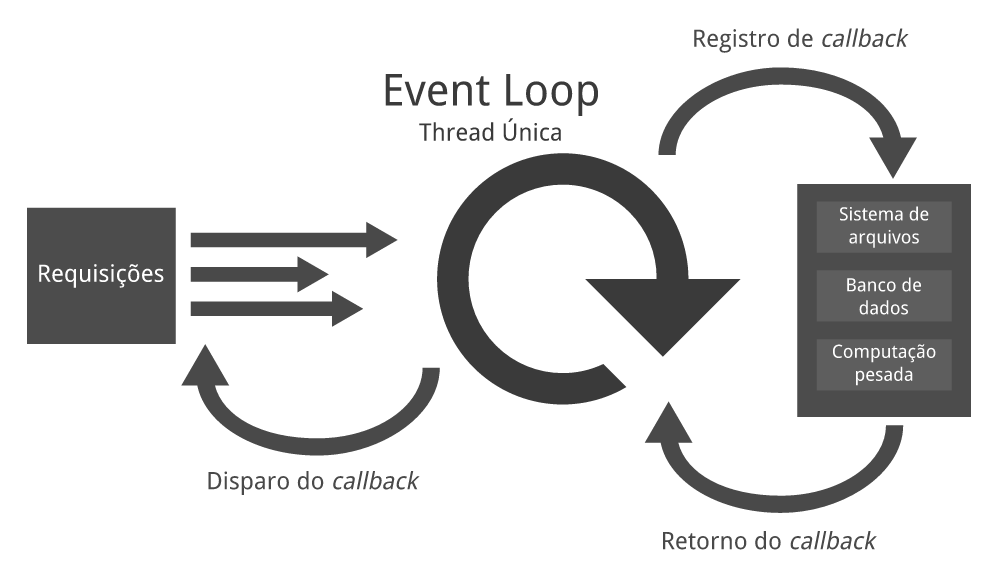
\includegraphics[scale=0.6]{imagens/node-eventloop.png}
	\caption{\small Fluxo simplificado de requisições no NodeJS. Fonte: maxroecker \cite{img-eventloop}}
	\label{fig:node-eventloop}
\end{figure}

Como se pode observar na figura, diferentemente dos servidores \textit{web} comuns, o NodeJS não cria um processo ou \textit{thread} para cada requisição que chega ao servidor. Ao invés disso, cada instância NodeJS é um processo que funciona como um \textit{event loop}, onde para cada operação de I/O requisitada, é registrada uma \textit{callback} que será chamada posteriormente no \textit{event loop} quando os dados estiverem disponíveis. Sendo assim, a thread principal nunca fica bloqueada, ela está sempre aguardando que um evento esteja para acontecer, que pode ser a chegada ou resposta de uma requisição, por exemplo. É possível que surjam questionamentos sobre como o NodeJS faz as requisições de I/O assíncronas e simultaneamente atende outras requisições, mas isso é abstraído ao desenvolvedor, pois o NodeJS utiliza um biblioteca multi-plataforma, codificada em C, chamada libuv \cite{libuv}, que trata as operações de I/O assincronamente com utilização de \textit{thread pool} e afins.

Tendo em mente todos esses conceitos do funcionamento da arquitetura do NodeJS, é possível entender o porque dele conseguir tratar muito mais conexões simultâneas do que as arquiteturas convencionais, pois a criação de processos e \textit{threads} tende a ser um recurso custoso para o sistema operacional, além de reservas de recursos valiosos do sistema, como memória RAM. É importante ressaltar que a programação assíncrona e o ambiente criado pelo NodeJS tem uma curva de aprendizado maior e se faz necessário maiores cuidados por parte do desenvolvedor, pois a utilização incorreta poderá acarretar no travamento da única \textit{thread} da instância da aplicação, bloqueando totalmente o sistema de processar novas requisições. 

Por outro lado, quando o entendimento é claro e o desenvolvimento é correto, a utilização dos recursos naturalmente é escalável e distribuída, pois a própria singularidade da plataforma nos faz trabalhar conceitos de sistemas distribuídos, como por exemplo, para que possamos aproveitar de todos os recursos de um processador multi-core com NodeJS, temos que executar mais de uma instância da aplicação, o que nos leva a trabalhar conceitos de clusterização, comunicação de processos e etc, o que facilita no escalonamento horizontal da aplicação em múltiplos servidores.

\subsection{NPM}
O NPM \cite{npm} é o gerenciador de pacotes do NodeJS. A função do NPM é oferecer um repositório central de qual se pode baixar diversos módulos distribuídos pela própria equipe que desenvolve o NodeJS ou que outros usuários tenham contribuído.

A evolução do NPM se tornou dominante, sendo considerado o maior repositório de registro de conteúdo Javascript do mundo. Devida a utilização do Javascript para outras finalidades além do desenvolvimento em NodeJS, muitos dos módulos disponibilizados pelo NPM não são parcialmente ou completamente desenvolvidos para a utilização com o NodeJS, sendo que muitos usuários e desenvolvedores utilizam e publicam conteúdo voltado para o desenvolvimento \textit{frontend}, que também utiliza o Javascript como principal linguagem. Talvez este seja um dos grandes motivos de sucesso do NPM em números.

Sua utilização é feita basicamente via linha de comando, onde iniciamos um novo repositório quando criamos uma aplicação, e apartir deste comando é criado um arquivo em formato JSON, chamado package.json, do qual ficará registrado todas as dependências daquele projeto, através da especificação do nome e versão de cada módulo baixado do repositório oficial.

A utilização de um gerenciador de pacotes traz diversos vantagens, dentre estas, a facilitação no versionamento de código, pois não é necessário manter uma cópia de um conteúdo que poderá ser baixado posteriormente de um local central, o controle das versões de cada biblioteca que se está utilizando no sistema, facilitando a resolução de problemas de compatibilidade e dependências uma das outras, local único para busca e contribuição de soluções na linguagem, entre outras.

\subsection{ExpressJS}
O ExpressJS \cite{expressjs} é o principal \textit{framework} NodeJS para desenvolvimento de aplicações \textit{web} e APIs. A sua proposta é ser simples, performático e \textit{loosely coupled} na construção de aplicações, sem interferir nas características padrões que o NodeJS oferece.

O desenvolvimento com o ExpressJS é bem intuitivo pela organização que ele propõe para a aplicação. Suas abstrações são apenas essenciais, que não interferem na utilização dos artifícios da própria linguagem nativa do NodeJS para a resolução dos problemas, sem muitas automatizações, sendo ainda mais conveniente oferecendo mecanismos de \textit{middlewares} que possibilitam total manipulação das requisições e seus atributos, injeção de \textit{template-engines} e outros \textit{handlers} e \textit{plugins} que podem ser baixados via NPM. A comunidade possui diversas soluções empregadas, o que também facilita na curva de aprendizado, produtividade e resolução de problemas. Rapidamente é possível instalá-lo na aplicação e se disponibilizar um servidor HTTP pronto para receber, tratar e responder requisições como API ou UI.

\subsection{SocketIO}
O SocketIO é uma biblioteca para a criação de aplicações tempo-real na \textit{web}, que permite troca de mensagens em formato binário ou texto de forma bi-direcional e instantânea. Ele funciona através de duas bases de código, uma aplicada no servidor NodeJS e outra no \textit{browser} do cliente. A biblioteca faz uso da tecnologia WebSocket para estabelecer uma comunicação bi-direcional e persistente entre servidor e cliente, mas em casos de problemas de compatibilidade, é utilizado o método de \textit{long polling} para estabelecer este tipo de comunicação. As bibliotecas do SocketIO utilizadas no servidor e no cliente possuem chamadas semelhantes, o que facilita na realização da interação dos dois lados.

A figura a seguir demonstra simplificadamente a forma de conexão entre servidor e cliente descrita anteriormente:

\begin{figure}[!htb]
	\centering
	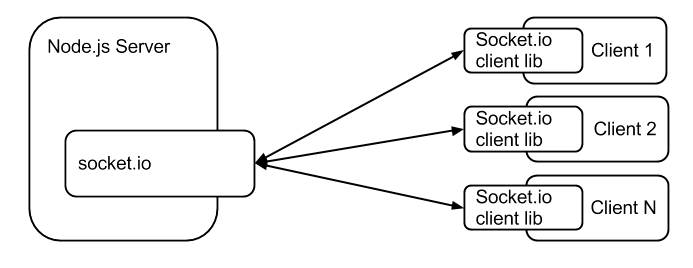
\includegraphics[scale=0.67]{imagens/socketio.png}
	\caption{\small Conexão entre servidor e cliente com SocketIO. Fonte: ifollow \cite{img-socketio}}
	\label{fig:socketio}
\end{figure}

Apesar do SocketIO ser um encapsulador da tecnologia \textit{websocket}, as chamadas de sua API são muito semelhantes a utilização do \textit{websocket} diretamente, onde a biblioteca apenas adiciona funcionalidades que são convenientes para o gerenciamento das conexões dos \textit{sockets}, como \textit{broadcast} de mensagens, atrelar informações específicas do usuário de cada \textit{socket}, entre outros.

A tecnologia \textit{websocket} é baseada em canais TCP, o que significa que os dados trafegados por ele tem a garantia de ordem e não perca de informações, o que torna a comunicação mais confiável e capaz de atender um abrangente número de necessidades. Também é preciso levar em conta os custos que canais TCP podem ter dependendo do tipo de dados que se quer transmitir, onde apesar da possibilidade de transmissão de conteúdo binário por \textit{websockets}, muitas das vezes é mais eficiente a utilização de um canal UDP, como faz uso a tecnologia WebRTC, que é muito utilizada para \textit{streaming} de vídeos, por exemplo.

\subsection{MongoDB}
O MongoDB é um banco de dados de alta performance, enquadrado nos conceitos de bancos de dados NoSQL. A escolha por este tipo de ferramenta se faz pelas características que o modelo de arquitetura escolhido traz para a aplicação. Os bancos de dados NoSQL foram criados para oferecer novas possibilidades para as demandas que exigem escalabilidade horizontal e performance na estrita e leitura de dados, o que se encaixa com os atributos das tecnologias da aplicação desenvolvida.

A forma como este tipo de banco de dados funciona remete diretamente aos ganhos de desempenho e escalabilidade, pois existe uma quebra de conceitos dos bancos de dados relacionais, como o ACID, que trazem flexibilidade em como se tratam os dados armazenados para se ter os benefícios citados. O MongoDB além de adotar estes conceitos, é um banco de dados orientado a documentos, onde a persistência dos dados é realizada em formato JSON. Apesar do conceito NoSQL ser uma grande ruptura de paradigmas, a maior parte da popularidade do MongoDB se deve a sua forma de interação com o usuário, que é amigável a quem está migrando dos conceitos relacionais para o modelo NoSQL. Apesar de não existir a necessidade de criação de tabelas, definição de relações, entre outros, a API do MongoDB oferece a criação de esquemas que remetem a conceitos parecidos, e também habilitam outras possibilidades, como a indexação de campos para buscas mais eficientes. As chamadas de busca no banco também são amigáveis, utilizando palavras chaves como \textit{SELECT, WHERE, ORDER BY}, entre outros. É importante salientar que algumas das funcionalidades citadas se devem ao uso de um modelador de dados chamado Mongoose \cite{mongoose}, ferramenta da qual oferece um \textit{set} de utilidades para se trabalhar com o MongoBD.
 
\subsection{Redis}
O Redis é um banco de dados NoSQL em memória, que implementa apenas alguns tipos de estruturas de dados, como \textit{strings, hashes, lists, sets} e \textit{sorted hashes}, e funcionalidades para gerência, busca e transmissão dos dados armazenados, o que o torna muito enxuto. Devido ao Redis ser um banco de dados que funciona em memória, seu desempenho é muito alto, tendo em vista que a memória RAM é um dos componentes de armazenamento de dados mais rápidos em leitura, escrita e transmissão na arquitetura computacional. Por outro lado, a memória RAM é volátil, o que nos leva a buscar entender qual a proposta de um banco de dados em memória.

A utilização principal do Redis é para servir como \textit{cache} e/ou \textit{message broker} de informações em sistemas. Em implementações \textit{stateless} o Redis pode servir como \textit{cache} de dados muito requisitados, pois seu rápido desempenho em memória pode ser vital para atender requisições em tempo hábil. Outra utilidade do Redis, que é o caso deste projeto, é do compartilhamento de dados entre servidores distintos de uma aplicação, onde através das estruturas de dados fornecidas pelo Redis e algumas funcionalidades, como a do protocolo PUB/SUB, é possível que se armazene dados no Redis e outra instância da aplicação sendo executada em outro local possa buscar estes mesmos dados. Devido a simplicidade e robustez que o Redis possui, uma única instância é capaz de realizar milhares de operações, aproximadamente 1.5 milhões por segundo \cite{redis-metrics}, podendo funcionar muito bem sendo este tipo de centralizador, pois o escalonamento de servidores de aplicação ocorre com muito mais frequência do que a de instâncias Redis. 

\section{Front-end}

\subsection{Bower}
O Bower \cite{bower} é um gerenciador de pacotes, assim como o NPM, mas com conteúdo focado para o \textit{frontend}. Através dele é possível fazer \textit{download} de diversas bibliotecas, como AngularJS, jQuery e Bootstrap. Sua utilização se dá através de linha de comando, onde ao criar um novo projeto \textit{frontend} o usuário deve iniciar o Bower no mesmo diretório, através de linha de comando, e este criará um arquivo chamado bower.json, que conterá informações do projeto e todas os nomes e versões de bibliotecas baixadas do seu repositório oficial, permitindo-se assim o gerenciamento de novos pacotes e resolução de dependências entre eles.

O NPM também oferece muitas das bibliotecas disponíveis no Bower, e o contrário muitas vezes não é válido, sendo assim, é comum a utilização dos dois gerenciadores de pacotes no projeto \textit{frontend}, o Bower e NPM.

\subsection{AngularJS}
O AngularJS \cite{angular} é um \textit{framework} Javascript para desenvolvimento de interfaces \textit{web}. Mais do que apenas interfaces, o AngularJS auxilia na criação de aplicações complexas no lado cliente da comunicação. Com o avanço das tecnologias e formas de se construir sistemas, ferramentas como o AngularJS vieram para ajudar na organização e qualidade dos sistemas que estavam se desenvolvendo.

A abordagem do AngularJS na construção de aplicações \textit{frontend} é completa, oferecendo suporte para manipulação do DOM, \textit{data binding}, gerenciamento de rotas, padrões de projeto (MVW, MVVM, MVC), entre outros. Apesar da fragmentação de alguns recursos em módulos separados, como as rotas, o produto AngularJS consegue oferecer uma solução completa para o desenvolvimento de interfaces de usuário.

O desenvolvimento de uma aplicação AngularJS, normalmente segue as diretivas de uma aplicação SPA com o estilo de programação declarativa, tendo em vista a forma com que se desenvolve interfaces para os \textit{browsers}, as tecnologias envolvidas, como o próprio HTML, em um ambiente orientado a eventos, se faz mais adequada este tipo de abordagem declarativa, que segue uma lógica mais comum as interfaces.

A arquitetura moldada ao um formato de API também é um fator determinante para a utilização de um \textit{framework} como o AngularJS, pois ele já oferece módulos e serviços para o consumo de dados através de \textit{endpoints} que forneçam dados em formato XML ou JSON.

\subsection{Angular Material}
O Angular Material \cite{angular-material} é uma outra solução do produto Angular, também para interfaces, mas focado em conceitos e características de \textit{design}, UX, reutilização, acessibilidade, compatibilidade \textit{cross-browsers}, responsividade, entre outros. 

A ferramenta oferece diversos componentes visuais de interface com efeitos e estilizações próprios, levando em conta diversos conceitos abstratos de \textit{design}, que enriquecem a experiência e agradabilidade do usuário ao ver e interagir com eles. Os componentes do Angular Material são totalmente compatíveis com as implementações AngularJS, facilitando na integração entre os componentes. Um grande problema que é evitado utilizando um \textit{framework} como este, são os de problemas de compatibilidade entre os diversos navegadores no mercado, onde cada um possui especificidades que podem causar comportamentos inesperados nos comentos de interface. Acessibilidade e outras otimizações também são importantes para a inclusão do site e SEO.

Por último, um benefício importante que o Angular Material dispõe, é o seu \textit{grid system}, baseado no CSS3 \textit{flexbox}. Esta característica possibilita que todo o conteúdo apresentado no site se redimensione de acordo com o tamanho da tela do dispositivo que está exibindo o conteúdo, possibilitando assim uma experiência viável para dispositivos móveis, do qual já citamos a importância em números \cite{internet-traffic-stats1} \cite{internet-traffic-stats2} \cite{internet-traffic-stats3}.  

\subsection{Gulp}
O Gulp \cite{gulp} é uma ferramenta de automatização de tarefas Javascript, comumente utilizado para automatizações de fluxos de trabalho no desenvolvimento \textit{frontend}. Sua utilização se dá por linha de comando e um arquivo de configuração chamado gulpfile.js. Neste arquivo Javascript podemos criar \textit{tasks} que irão realizar tarefas diversas, de acordo com a programação realiza, como por exemplo a execução de testes unitários, concatenação e minificação de arquivos, compilação de linguagens intermediárias, como o SASS, \textit{autoprefixer}, \textit{lint}, entre outros.

Existem diversos \textit{plugins} disponíveis no NPM que executam tarefas específicas, como as citadas anteriormente, bastando ao usuário baixá-las e chamá-las em suas \textit{tasks}, que podem executar uma ou mais funcionalidades organizadas através de chamadas síncronas pelo método pipe de cada \textit{task}.

\subsection{SASS}
O SASS \cite{sass} é uma linguagem de \textit{script} que pode ser interpretada para CSS. O CSS tem uma sintaxe muito simples e com poucas funcionalidades para estruturação, reaproveitamento e modularizarão de código, onde o SASS oferece uma série de funcionalidades, como variáveis, operadores, herança e modularização, que podem ser aplicadas para a geração de folhas de estilos.

Todas as funcionalidades do SASS facilitam a construção de interfaces complexas, onde se exigem muitos componentes, classes, hierarquização de seletores, entre outros. A interpretação do código SASS para CSS pode ser feita por diversos interpretadores, inclusive o próprio Gulp oferece \textit{plugins} para este fim.

\subsection{HAML}


\subsection{Webpack}


\subsection{Babel}


\subsection{Nginx}